\chapter{Electronic many-body problem}\label{chap:electrons}

{\sffamily This chapter briefly reviews those basic building blocks of the electronic structure theory that are necessary for the presentation of the actual new work done for this thesis.
This comprises mostly the density functional theory, the adiabatic-connection fluctuation--dissipation framework, and the theory of the nonlocal dipole polarizability.
}

\section{Schrödinger equation}

The role of the second Newton law ($\mathrm d^2\mathbf r/\mathrm dt^2=\mathbf F/m$) in nonrelativistic quantum mechanics is played by the Schrödinger equation, which therefore underlies all material discussed in this thesis.
In quantum mechanics, the state of a fixed number, $N$, of electrons in a molecule or a crystal is fully specified by a vector, $|\Psi\rangle$, from the $N$-electron Hilbert space.
Measurable properties of the state, such as energy, are expressed as Hermitian operators, whose eigenvalues are the possibly measured values of the property, the eigenvectors form a complete orthogonal basis of the Hilbert space, and the probability of measuring an eigenvalue corresponding to a given eigenvector is given by the square of the inner product of that eigenvector and the given state.
The operator for energy, called Hamiltonian, $\hat H$, has a central role in quantum mechanics because it determines time evolution of the state via the Schrödinger equation,
\begin{equation}
  \frac{\partial|\Psi\rangle}{\partial t}=-\mathrm i\hat H|\Psi\rangle
  \makebox[0pt]{\hspace{0.4\linewidth}(in a.\,u.)}
  \label{eq:schrodinger-time}
\end{equation}
This equation dictates that the phases of components of a state corresponding to different energy eigenstates oscillate at different rates, and eventually appear to be random for a system in equilibrium with its environment, so that one can regard the system as an ensemble of eigenstates of the Hamiltonian.
Because the probability of the $n$-th eigenstate ($n=0,1,\ldots$) with energy $E_n$ at temperature $T$ is proportional to $\exp(-E_n/T)$, and because the energy differences between electronic energy eigenstates typically count in at least thousands of kelvins ($1\,\mathrm{eV}\doteq12\,000\,\mathrm{K}$ in atomic units), most matter on Earth is found in the electronic ground state.

The nonrelativistic Hamiltonian for $N$ electrons ($i=1,\ldots,N$) in electric potential $v_\text{ext}(\mathbf r)$ consists of three terms that correspond to the kinetic energy, potential energy, and interelectronic Coulomb repulsion,
\begin{equation}
  \hat H=\sum_i\frac{\mathbf{\hat p}_i^2}2-\sum_i v_\text{ext}(\mathbf{\hat r}_i)+\sum_{i<j}\frac1{|\mathbf{\hat r}_i-\mathbf{\hat r}_j|}\equiv\hat T+\hat V_\text{ext}+\hat V_{ee}
  \label{eq:el-hamiltonian}
\end{equation}
Because electrons are fermions (particles with half-integer spin), the corresponding Hilbert space is antisymmetric, meaning that when any two electrons are exchanged, the resulting state vector must be equal to the negative of the original state vector.
In a free molecule or crystal, the nuclei at positions $\mathbf R_A$ with charges $q_A$ generate the external potential for the electrons,
\begin{equation}
  v_\text{ext}(\mathbf r)=\sum_A\frac{q_A}{|\mathbf r-\mathbf R_A|}
\end{equation}
In the basis of eigenstates of the position operators, $\mathbf{\hat r}_i$, and spin operators, $\hat s_i$, one can define a wave function, $\Psi(\{\mathbf r_i s_i\})=\langle\mathbf r_i s_i|\cdots\langle\mathbf r_N s_N|\Psi\rangle$, and the search for eigenvectors is then turned into a differential equation,
\begin{equation}
  \left(-\sum_i\frac{\boldsymbol\nabla_i^2}2-\sum_i\sum_A\frac{q_A}{|\mathbf r_i-\mathbf R_A|}+\sum_{i<j}\frac1{|\mathbf r_i-\mathbf r_j|}-E\right)\Psi(\mathbf r_1 s_1,\ldots,\mathbf r_N s_N)=0
\end{equation}
The wave function must be antisymmetric, and the solution of the equation gives possible values of the electronic energy, $E$, which are the eigenvalues of the Hamiltonian.
This equation cannot be solved analytically already for the simplest of systems, and formulating approximate, efficient, yet accurate methods for its solution is historically the biggest problem in quantum chemistry.

The spin variables are discrete ($s_i\in\{-\frac12,\frac12\}$), and because we operate in nonrelativistic quantum mechanics, they do not enter the Hamiltonian, but only influence the form of the spatial dependence of the wave function via the requirement of the antisymmetry~\cite{Pauncz79}.
The spin part of the wave function can be always written in terms of the one-electron spin functions, $\uparrow\!(s)$ and $\downarrow\!(s)$, whose values are either zero or one,
\begin{equation}
\begin{aligned}
  \uparrow\!(\tfrac12)&=1 & \downarrow\!(\tfrac12)&=0 \\
  \uparrow\!(-\tfrac12)&=0 & \downarrow\!(-\tfrac12)&=1
\end{aligned}
\end{equation}
Because of the antisymmetry, the probability of finding two electrons of the same spin at the same position is zero, $\Psi(\mathbf rs,\mathbf rs,\ldots)=0$, which is also called the Pauli exclusion principle.

\section{Variational method and energy functionals}

One of the oldest approaches to finding the ground state, but also a foundation of many modern methods, is based on the fact that the eigenstates of the Hamiltonian, $|\psi_n\rangle$, form a complete basis,
\begin{equation}
\begin{aligned}
  \langle\Psi|\hat H|\Psi\rangle
  &=\langle\Psi|\hat H\sum_n|\psi_n\rangle\langle\psi_n|\Psi\rangle
  =\sum_n E_n\langle\Psi|\psi_n\rangle\langle\psi_n|\Psi\rangle \\
  &\geq E_0\sum_n\langle\Psi|\psi_n\rangle\langle\psi_n|\Psi\rangle=E_0\langle\Psi|\Psi\rangle=E_0
\end{aligned}
\end{equation}
As a result, the expectation value of the Hamiltonian is never smaller than the ground-state energy, and if the energy is understood as a functional of a wave function, $E[\Psi]$, the ground state can be found at its minimum,
\begin{equation}
  |\psi_0\rangle=\operatorname*{arg\,min}_{|\Psi\rangle}E[\Psi]
  \label{eq:minimization}
\end{equation}
(In fact all eigenstates can be gradually found in this fashion, by requiring that they are orthogonal to all the lower-energy eigenstates.)

Because all terms in the Hamiltonian are either one- or two-electron, do not depend on spin, and the wave function is antisymmetric, the expression for the energy functional can be simplified by partial integrations over $\Psi$~\cite{Parr89},
\begin{equation}
  E[\Psi]=\int\mathrm d\mathbf r\,\big(-\tfrac12\boldsymbol\nabla_{\mathbf r'}^2 \gamma(\mathbf r,\mathbf r')\!\big)\big|_{\mathbf r'=\mathbf r}+\int\mathrm d\mathbf r\,v_\text{ext}(\mathbf r)n(\mathbf r)+\frac12\iint\mathrm d\mathbf r_1\mathrm d\mathbf r_2\frac{n_2(\mathbf r_1,\mathbf r_2)}{|\mathbf r_1-\mathbf r_2|}
  \label{eq:master-energy-functional}
\end{equation}
The energy is then expressed in terms of the first-order density matrix, $\gamma(\mathbf r,\mathbf r')$, the electron-pair density, $n_2(\mathbf r_1,\mathbf r_2)$, and the electron density, $n(\mathbf r)=\gamma(\mathbf r,\mathbf r)$.
In principle, the ground-state energy can be found just as well by minimizing this energy functional over all $n$, $\gamma$, and $n_2$ that originate from the same wave function.
But this latter search constraint, called the $N$-representability problem, is what makes this approach unfeasible, because the sufficient conditions for $n_2$ to be $N$-representable are unknown.\footnote{
More precisely, the energy functional is a functional of the second-order density matrix, $\gamma_2(\mathbf r_1\mathbf r_2,\mathbf r'_1\mathbf r'_2)$, from which $n_2(\mathbf r_1,\mathbf r_2)=2\gamma_2(\mathbf r_1\mathbf r_2,\mathbf r_1\mathbf r_2)$ and $\gamma_1(\mathbf r,\mathbf r')=2\int\mathrm d\mathbf r_2\gamma_2(\mathbf r\mathbf r_2,\mathbf r'\mathbf r_2)/(N-1)$, and it is $\gamma_2$ for which the sufficient $N$-representability conditions are not known.
}
The electron-pair density can be written in terms of the electron density and a pair correlation (distribution) function, $g(\mathbf r_1,\mathbf r_2)$,
\begin{equation}
  n_2(\mathbf r_1,\mathbf r_2)=n(\mathbf r_1)n(\mathbf r_2)g(\mathbf r_1,\mathbf r_2)
\end{equation}
If the motions of the electrons were uncorrelated, the pair correlation function would be equal to 1, but in reality the wave-function antisymmetry and the interelectronic Coulomb term cause it to deviate from 1.
By using $g=1-(1-g)$, the interelectronic energy term can be naturally split into a classical part (also called the Hartree energy), which is simply the electrostatic energy, $J[n]$, of the electron charge density, and a nonclassical correction,
\begin{equation}
  \langle\Psi|\hat V_{ee}|\Psi\rangle=J[n]-
  \frac12\iint\mathrm d\mathbf r_1\mathrm d\mathbf r_2\frac{n(\mathbf r_1)n(\mathbf r_2)}{|\mathbf r_1-\mathbf r_2|}\big(1-g(\mathbf r_1,\mathbf r_2)\!\big)
\end{equation}
The total electronic energy can then be written as a sum of four terms,
\begin{equation}
  E[\Psi]=T[\gamma]+V_\text{ext}[n]+J[n]+\text{nonclassical term}
  \label{eq:energy-nonclassical}
\end{equation}

\section{Mean-field models}

Unlike the spin part of the wave function, the spatial part cannot be in general expressed in terms of one-electron functions because of the Coulomb force between electrons.
For instance, the ground state of harmonium, a two-electron system described by the Hamiltonian in~\eqref{eq:el-hamiltonian} with $v_\text{ext}(\mathbf r)=r^2/8$, has the form
\begin{equation}
  \psi_0(\mathbf r_1s_1,\mathbf r_2s_2)\sim\big(1+\tfrac12|\mathbf r_1-\mathbf r_2|\big)\exp\big(-\tfrac14(r_1^2+r_2^2)\big)(\uparrow\downarrow-\downarrow\uparrow)
\end{equation}
The simple prefactor $(1+\frac12 r_{12})$ is caused by the Coulomb term, and makes the two electrons more likely to be found far apart than close to each other.
In contrast to the Pauli principle though, the Coulomb term is not strong enough to make the electrons completely avoid each other, and $\psi_0(\mathbf r,\mathbf r)\neq0$.
Unfortunately, harmonium is the only many-electron system with a known exact wave function in a closed form, and realistic calculations of common systems require approximate models.

\begin{figure}
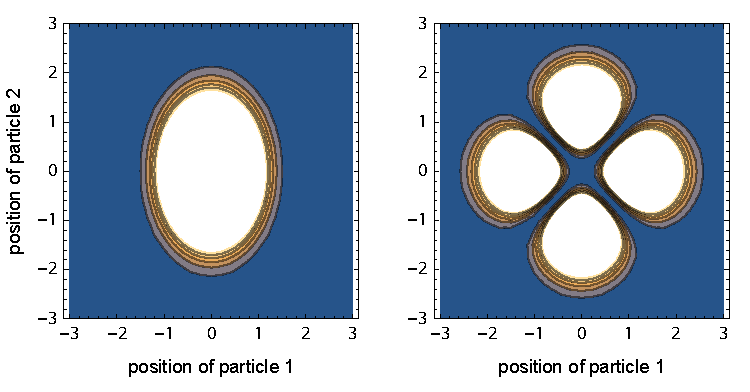
\includegraphics[center]{media/exchange.pdf}
\caption{\textbf{Antisymmetrization.}
Contour plots of the square of a wave function, $|\Psi(x_1,x_2)|^2$, of two particles in one dimension formed from two one-particle functions, $\phi_1(x)=\exp(-x^2)$ and $\phi_2(x)=\exp(-x^2/2)$.
On the left, $\Psi$ is a simple product.
On the right, $\Psi$ is an antisymmetrized product, $\phi_1(x_1)\phi_2(x_2)-\phi_1(x_2)\phi_2(x_1)$.
The contour levels in both plots are equal.
}\label{fig:exchange}
\end{figure}

Although true many-electron wave functions cannot be built from one-electron functions (also called orbitals), such constructs form the basis of almost all approximate electron models.
An antisymmetrized product of spin-orbitals, $\phi_j(\mathbf r_i s_i)$, is called a Slater determinant, $\mathcal D(\{\phi_j\})$, and the approximate many-electron wave function thus formed is characterized by a simple expression for the one-electron density matrix, $\gamma(\mathbf r,\mathbf r')=\sum_{s}\sum_j f_j\phi_j^*(\mathbf rs)\phi_j(\mathbf r's)$, in which $f_j\in\{0,1\}$ are the occupation numbers of the orbitals.
(Generalizing from here, any $N$-representable density matrix can be expressed in this form by allowing any $0\leq f_j\leq1$.)
Minimizing $E[\Psi]$ with respect to this Slater-type wave function is called the Hartree--Fock (HF) approximation.
The antisymmetrization of same-spin electrons works on the spatial part of the wave function (Fig.~\ref{fig:exchange}), and of opposite-spin electrons on the spin part.
As a result of this, the pair correlation function for opposite-spin electrons in a Slater determinant is equal to 1, whereas that of the same-spin electrons is modified ($n^\uparrow=n^\downarrow=n/2$ for simplicity),
\begin{equation}
  g^{\uparrow\uparrow}(\mathbf r_1,\mathbf r_2)=g^{\downarrow\downarrow}(\mathbf r_1,\mathbf r_2)=1-\frac{|\gamma(\mathbf r_1,\mathbf r_2)|^2}{n(\mathbf r_1)n(\mathbf r_2)}\qquad
  g^{\uparrow\downarrow}(\mathbf r_1,\mathbf r_2)=1
\end{equation}
In line with the Pauli principle, the pair correlation function of same-spin electrons in the HF model starts at zero when $\mathbf r_1$ equals $\mathbf r_2$, but then goes quickly to 1, around which it slowly oscillates with decreasing amplitude as $r_{12}$ increases.
(In sodium, for instance, $g$ reaches 0.99 already at $|\mathbf r_1-\mathbf r_2|\approx 0.25$\,\AA.)

The modification of $g$ from 1 due to the antisymmetry reduces the short-range repulsion between same-spin electrons, and this part of the nonclassical term in~\eqref{eq:energy-nonclassical} is called the exchange energy,
\begin{equation}
  K[\gamma]=-\frac14\iint\mathrm d\mathbf r_1\mathrm d\mathbf r_2\frac{|\gamma(\mathbf r_1,\mathbf r_2)|^2}{|\mathbf r_1-\mathbf r_2|}
\end{equation}
When incorporated into the exact energy functional, the remaining part of the electronic energy is called the correlation energy (despite the fact that the exchange energy also originates from a nontrivial pair correlation function),
\begin{equation}
  E[\Psi]=T[\gamma]+V_\text{ext}[n]+J[n]+K[\gamma]+\text{correlation}
  \label{eq:energy-with-exchange}
\end{equation}
Omitting the correlation part and minimizing this functional with respect to all $N$-representable density matrices ($f_j\in\{0,1\}$ is obtained as a result) leads to the HF one-electron equations, which describe the motion of an electron in the mean field generated by all the other electrons (hence then name ``mean-field'' methods).
In most molecules and nonconducting solids, the basic structure of the ground-state wave function is dominated by the kinetic energy, and the HF approximation works quite well in such cases, failing only quantitatively to account for the opposite-spin correlation and the small Coulomb correction to the same-spin correlation.
Still, two fundamental problems exist:
First, the Coulomb interaction becomes as important as the kinetic energy for the wave-function structure\footnote{
More precisely, the functional derivatives of the Coulomb energy and the kinetic energy with respect to the wave function become equally important.}
in metals, certain special materials (such as Mott insulators), and spin-unpaired (open-shell) systems, and the missing opposite-spin correlation leads to qualitatively wrong wave functions in such cases.
For instance, it leads to spurious preference to ``cluster'' same-spin electrons together, leading to the formation of unphysical spin waves in metals in the HF approximation~\cite{OverhauserPR62}.
Second, the long-range finer structure of the wave function is dominated by the Coulomb interaction, not by the antisymmetry, leading to complete neglect of vdW interactions in the HF approximation.

Approximating the correlation energy as a functional of the one-electron density matrix and minimizing that functional with respect to $\gamma$ leads to the density-matrix functional theory (of which the HF method is a special case).
Going further, the post-HF methods of quantum chemistry construct more complex wave functions on top of the Slater determinant, and approximate the correlation energy either by reapplying the variational technique or using the perturbation theory with the correlation term in the functional being the perturbation.
Using linear combinations of Slater determinants instead of a single one leads to the class of multi-configurational methods.

\section{Diffusion quantum Monte Carlo}\label{sec:dqmc}

The diffusion quantum Monte Carlo (DQMC) is a practical numerical method to calculate the exact electronic ground-state energy that uses the mean-field wave functions of the previous section only indirectly~\cite{FoulkesRMP01}.
Calculations performed for this thesis use it indirectly via the parametrization of effective electron models introduced below, as well as directly to calculate reference binding energies in Chapter~\ref{chap:pi-pi}.

DQMC is based on the fact that the imaginary-time evolution operator of~\eqref{eq:schrodinger-time} projects out the true ground state in the limit of the infinite time because the excited states have a higher energy and decay faster,
\begin{equation}
  \exp(-\tau\hat H)|\Psi\rangle=\sum_n\exp(-\tau E_n)|\psi_n\rangle\xrightarrow{\tau\rightarrow\infty}\exp(-\tau E_0)|\psi_0\rangle
  \label{eq:dqmc}
\end{equation}
This fact becomes numerically useful by reinterpreting the corresponding wave function as a distribution of particles and the evolution operator as describing a stochastic diffusion-and-branching process of these particles.
(In fact, this process can also be interpreted as a stochastic gradient-descent minimization of the Hamiltonian expectation value, directly connecting DQMC to the standard variational techniques~\cite{SchwarzPRL17}.)
The ground-state wave function and energy can then be obtained by stochastically evolving the particles with $\exp(-\tau(\hat H-E))$, while adjusting $E$ such that the number of the particles is kept constant, so that $E$ eventually converges to $E_0$.
Ending the evolution process before infinite time gives the wave function and energy with some limited, but statistically known and arbitrarily good accuracy.
The correspondence between the wave function and the particle distribution is only valid when the wave function is positive everywhere.
This is true for the ground state of distinguishable or bosonic particles, but not for the ground state of fermions (electrons), which must be antisymmetric (for more than one particle).
This makes direct application of DQMC to electrons impractical without further approximations.

The $(3N-1)$-dimensional plane of points at which the wave function of $N$ electrons is zero is called the nodal surface.
In general, it is no less complicated than the full wave function, and the $(3N-3)$-dimensional coincidence plane at which $\mathbf r_i=\mathbf r_j$ and $\Psi=0$ by antisymmetry forms only its lower-dimensional scaffold~\cite{CeperleyJSP91}.
If the nodal surface of the ground-state wave function was known, the full wave function could be recovered by running a DQMC simulation independently in each nodal pocket, in which the wave function does not change sign.
The fixed-node approximation then uses the nodal surface of some approximate wave function to determine these independent DQMC simulations.
Because this effectively restricts the wave function to a certain form, the obtained approximate ground-state energy is variationally guaranteed to be higher than the true energy.

Modified Slater-type wave functions obtained from mean-field methods (either HF or KS-DFT, described below) are usually used to determine the nodal surface in the fixed-node approximation.
The missing correlation (in the sense of a pair correlation function) in the Slater determinant, $\mathcal D$, due to the Coulomb interaction is added in an ad-hoc way via the so-called Jastrow factor, $\mathcal J$,
\begin{equation}
\begin{gathered}
  \Psi(\{\mathbf r_i s_i\})=\exp\big(\mathcal J(\{\mathbf r_i s_i\})\!\big)\mathcal D(\{\mathbf r_i s_i\}) \\
  J(\{\mathbf r_i s_i\})=\sum_i u_1(\mathbf r_i s_i)+\sum_{i<j} u_2(\mathbf r_i s_i,\mathbf r_j s_j)
\end{gathered}
\end{equation}
The two-electron Jastrow functions, $u_2$, decrease the probability of two electrons coming close to each other (different for same- and opposite-spin electron pair), while the one-electron functions, $u_1$, restore the electron density of $\mathcal D$ that would be otherwise somewhat diffused by the two-electron Jastrow functions.
The particular forms of $u_1$ and $u_2$ are mostly a result of experimentations and can be found for instance in~\cite{FoulkesRMP01}.

\section{Density-functional theory}

The theoretical framework presented in this section has led to the most widely used methods for calculating the electronic structure of molecules and materials, and it is the lack of vdW interactions in its most popular approximations that renewed the theoretical interest in vdW interactions.
It provides the context, motivation, as well as essential tools for most of the work in this thesis.

One can try to go one step further from the density-matrix functional theory, and express the electronic energy in terms of the electron density only, resulting in the density-functional theory (DFT).
That this is in principle possible was shown by \citet{HohenbergPR64} and later more rigorously by \citet{LevyPNAS79}, who divided the minimization in~\eqref{eq:minimization} over all antisymmetric wave functions in two steps, one over wave functions with a given density, the other over all densities, thus establishing the Hohenberg--Kohn functional, $F_\text{HK}$,
\begin{equation}
\begin{aligned}
  E_0&=\min_\Psi E[\Psi]=\min_n\min_{\Psi\rightarrow n}E[\Psi]=\min_n\big(\min_{\Psi\rightarrow n}(T[\Psi]+V_{ee}[\Psi])+V_\text{ext}[n]\big) \\
  &\equiv\min_n(F_\text{HK}[n]+V_\text{ext}[n])\equiv\min_n(E[n])
\end{aligned}
\end{equation}
If a given input density of the Hohenberg--Kohn functional, $F_\text{HK}$, is $v$-representable, meaning that there is some external potential (other than $V_\text{ext}$) of which ground state has that density, then the minimizing wave function, $\Psi_\text{HK}$, is the ground state for the corresponding external potential.
For densities that are not $v$-representable, the HK functional is still well-defined.
In either case, one can define the kinetic-energy functional, $T[n]\equiv T[\Psi_\text{HK}]$, and $V_{ee}[n]\equiv V_{ee}[\Psi_\text{HK}]$.
The task of DFT is then to devise sufficiently accurate approximations to $T[n]$ and $V_{ee}[n]$.
(The theory can be equivalently formulated using the electron spin densities, $n_\uparrow(\mathbf r)$ and $n_\downarrow(\mathbf r)$, which gives a more useful framework for approximations in the case of spin-polarized systems.)

Historically, the development of DFT was hampered by unsuccessful attempts at the kinetic-energy functional, whose various approximate formulations explicitly in terms of the electron density fail to reproduce any electronic shell structure in atoms.
This problem was largely solved by \citet{KohnPR65}, KS, who approximated the true kinetic energy with that of an auxiliary system of noninteracting electrons ($V_{ee}=0$) having the same density as the actual system,
\begin{equation}
\begin{aligned}
  T[n]&=T[\Psi_\text{HK}]=T\big[\operatorname*{arg\,min}_{\Psi\rightarrow n}(T[\Psi]+V_{ee}[\Psi])\big] \\
  &\approx T\big[\operatorname*{arg\,min}_{\Psi\rightarrow n}T[\Psi]\big]=\min_{\Psi\rightarrow n}T[\Psi]\equiv T_\text{s}[n]
\end{aligned}
\label{eq:ks-kinetic}
\end{equation}
The wave function minimizing $T_\text{s}$, $\Psi_\text{s}$, is always of the Slater type, and would in fact be a ground state of the noninteracting system if it was put in a particular external potential, called the KS potential,\footnote{
More precisely, it would be a ground state only if the given density is noninteracting $v$-representable, otherwise it would be an excited state.
}
\begin{equation}
  v_\text{s}(\mathbf r)=-\frac{\delta T_\text{s}[n]}{\delta n(\mathbf r)}
\end{equation}
After the KS approximation, the remaining unknown terms are collected in the so-called exchange--correlation (XC) functional (so named despite the contained kinetic-energy correction),
\begin{equation}
\begin{aligned}
  E[n]&=T_\text{s}[n]+V_\text{ext}[n]+J[n]+(T[n]-T_\text{s}[n]+V_{ee}[n]-J[n]) \\
  &\equiv T_\text{s}[n]+V_\text{ext}[n]+J[n]+E_\text{xc}[n]
  \label{eq:ks-dft-energy}
\end{aligned}
\end{equation}
The aim of KS-DFT is then to search for approximate formulations of $E_\text{xc}$ expressed explicitly in terms of the electron density.

Minimization of this functional with respect to $N$-representable densities leads to the KS one-electron equations (another mean-field model, but unlike the HF model, exact in principle), whose structure differs from the HF equations mathematically only in that their effective mean-field potential is local rather than nonlocal,
\begin{equation}
\begin{aligned}
  v_\text{xc}(\mathbf r)&=v_\text{ext}(\mathbf r)+\frac{\delta(J[n]+E_\text{xc}[n])}{\delta n(\mathbf r)} \\
  v_\text{HF}(\mathbf r,\mathbf r')&=\left(v_\text{ext}(\mathbf r)+\frac{\delta J[n]}{\delta n(\mathbf r)}\right)\delta(\mathbf r-\mathbf r')+\frac{\delta K[\gamma]}{\delta\gamma(\mathbf r,\mathbf r')}
\end{aligned}
\end{equation}
This difference makes the KS equations somewhat less complex, and more efficient to solve numerically, which is one of the reasons for the popularity of KS-DFT over the HF method.
At the minimum of $E[n]$, the effective-mean field potential of the KS equations, $v_\text{xc}(\mathbf r)$, is equal to the KS potential of the auxiliary noninteracting system, $v_\text{s}(\mathbf r)$.

\section{Adiabatic-connection fluctuation--dissipation theorem}

This section introduces the starting point for the classification of vdW methods presented in Chapter~\ref{chap:vdw-methods}.
The auxiliary KS system of noninteracting electrons can be adiabatically connected to the real system by slowly turning on the interelectronic Coulomb interaction, $\lambda\hat V_{ee}$, from $\lambda=0$ to $\lambda=1$, while keeping the electron density constant by adjusting the Kohn--Sham potential.
\begin{equation}
\begin{gathered}
  F_\text{HK}(\lambda)[n]=\min_{\Psi\rightarrow n}(T[\Psi]+\lambda V_{ee}[\Psi])\qquad
  v_\text{s}(\mathbf r;\lambda)=-\frac{\delta F_\text{HK}(\lambda)[n]}{\delta n(\mathbf r)} \\
  E(\lambda)[n]=F_\text{HK}(\lambda)[n]+V_\text{s}(\lambda)[n]
\end{gathered}
\end{equation}
The standard HK functional and KS potential are recovered for $\lambda=1$ and $\lambda=0$, respectively, whereas the Kohn--Sham potential for the true system reduces to the external potential, $V_\text{s}(1)[n]=V_\text{ext}[n]$.
The true electronic energy ($\lambda=1$) can be obtained from the noninteracting energy ($T_\text{s}[n]+V_\text{s}[n]$) by integrating over $\mathrm dE/\mathrm d\lambda$,
\begin{equation}
  E(1)[n]=E(0)[n]+\int_0^1\mathrm d\lambda\frac{\mathrm d E(\lambda)[n]}{\mathrm d\lambda}
  \label{eq:adiabatic-connection}
\end{equation}
Because the process is adiabatic, the system is in the ground state at any point, so the HK functional is stationary with respect to the wave function of the system ($\delta F_\text{HK}/\delta\Psi=0$), and the expression for $\mathrm dE/\mathrm d\lambda$ reduces to a simple formula (this is also called the Hellmann--Feynman theorem),
\begin{equation}
\begin{aligned}
  \frac{\mathrm d E(\lambda)[n]}{\mathrm d\lambda}&=\frac{\partial F_\text{HK}(\lambda)}{\partial\lambda}[\Psi_\text{HK}(\lambda)]+\frac{\delta F_\text{HK}(\lambda)[\Psi]}{\delta\Psi}\Bigg|_{\Psi=\Psi_\text{HK}(\lambda)}\frac{\partial\Psi_\text{HK}(\lambda)}{\partial\lambda}+\frac{\mathrm dV_s(\lambda)[n]}{\mathrm d\lambda} \\
  &=V_{ee}[\Psi_\text{HK}(\lambda)]+\frac{\mathrm dV_s(\lambda)[n]}{\mathrm d\lambda}
\end{aligned}
\end{equation}
Inserting the derivative into~\eqref{eq:adiabatic-connection}, one gets an alternative expression for the electronic energy that provides, by comparison to~\eqref{eq:ks-dft-energy}, an explicit formula for the XC energy (the last term),
\begin{equation}
\begin{aligned}
  E(1)[n]&=T_\text{s}[n]+V_\text{s}(0)[n]+\int_0^1\mathrm d\lambda V_{ee}[\Psi_\text{HK}(\lambda)]+V_\text{s}(1)[n]-V_\text{s}(0)[n] \\
  &=T_\text{s}[n]+V_\text{ext}[n]+J[n]-\int_0^1\mathrm d\lambda\,\frac12\iint\mathrm d\mathbf r_1\mathrm d\mathbf r_2\frac{n(\mathbf r_1)n(\mathbf r_2)-n_2(\mathbf r_1,\mathbf r_2;\lambda)}{|\mathbf r_1-\mathbf r_2|}
  \label{eq:energy-adiabatic}
\end{aligned}
\end{equation}

The fluctuation--dissipation theorem is a deep result of (quantum) statistical physics that relates correlations in fluctuations of any physical quantity describing a system in equilibrium with the dissipative part of the nonequilibrium response of that quantity to an external perturbation of the system~\cite{CallenPR51}.
The linear density response function, $\chi$, of an electronic system describes the change in the electron density at time $t$ generated by a change in the external potential at time $t'<t$,
\begin{equation}
  \frac{\delta n(\mathbf r,t)}{\delta v_\text{ext}(\mathbf r',t')}=\chi(\mathbf r,\mathbf r',t-t')
\end{equation}
It is often more convenient to Fourier-transform the time to frequency, $u$,
\begin{equation}
  \frac{\delta n(\mathbf r,u)}{\delta v_\text{ext}(\mathbf r',u)}=\chi(\mathbf r,\mathbf r',u)
\end{equation}

A particular version of the fluctuation--dissipation theorem for the fluctuations of the electron density then enables one to express the electron-pair density, $n_2$, in terms of the density response.
This version of the theorem, at zero temperature, is expressed in terms of the density operator, $\hat n(\mathbf r)=\sum_i\delta(\mathbf r-\mathbf r_i)$, (see \citealp[eq.~4.8]{CallenPR51}, \citealp[eq.~124.10]{Landau80}, \citealp[eq.~8.6.2]{Parr89}, and \citealp[eq.~8]{KohnPRL98}),
\begin{equation}
  \langle\Psi|(\hat n(\mathbf r_1)-n(\mathbf r_1)\!)(\hat n(\mathbf r_2)-n(\mathbf r_2)\!)|\Psi\rangle=-\frac1\pi\int_0^\infty\mathrm du\operatorname{Im}\chi(\mathbf r_1,\mathbf r_2,u)
\end{equation}
The electron-pair density can be likewise expressed in terms of the density operators,
\begin{equation}
  n_2(\mathbf r_1,\mathbf r_2)=\langle\Psi|\hat n(\mathbf r_1)\hat n(\mathbf r_2)-\hat n(\mathbf r_1)\delta(\mathbf r_1-\mathbf r_2)|\Psi\rangle
\end{equation}
With the help of following identity,
\begin{equation}
  \langle\Psi|(\hat n(\mathbf r_1)-n(\mathbf r_1)\!)(\hat n(\mathbf r_2)-n(\mathbf r_2)\!)|\Psi\rangle \\
  =\langle\Psi|\hat n(\mathbf r_1)\hat n(\mathbf r_2)|\Psi\rangle-n(\mathbf r_1)n(\mathbf r_2)
\end{equation}
one can finally relate $n_2$ and $\chi$,
\begin{equation}
  n(\mathbf r_1)n(\mathbf r_2)-n_2(\mathbf r_1,\mathbf r_2)=\frac1\pi\int_0^\infty\mathrm du\operatorname{Im}\chi(\mathbf r_1,\mathbf r_2,u)+n(\mathbf r_1)\delta(\mathbf r_1-\mathbf r_2)
  \label{eq:fluctuation-dissipation}
\end{equation}
In this equation, the left-hand side is finite for $\mathbf r_1=\mathbf r_2$, and the divergent second term on the right-hand side is formally canceled by the divergence of the response function at $\mathbf r_1=\mathbf r_2$.
Plugging this equation into~\eqref{eq:energy-adiabatic}, the XC energy is expressed in terms of the density response function,
\begin{equation}
  E_\text{xc}[\chi]=-\int_0^1\mathrm d\lambda\,\frac12\iint\mathrm d\mathbf r_1\mathrm d\mathbf r_2\frac{\frac1\pi\int_0^\infty\mathrm du\operatorname{Im}\chi(\mathbf r_1,\mathbf r_2,u;\lambda)+n(\mathbf r_1)\delta(\mathbf r_1-\mathbf r_2)}{|\mathbf r_1-\mathbf r_2|}
\end{equation}
A standard form of the adiabatic-connection fluctuation--dissipation (ACFD) formula is reached by introducing the Coulomb operator, $v(R)\equiv1/R$, and using the Wick rotation, $\int_0^\infty\mathrm du\operatorname{Im}\chi(u)=\int_0^\infty\mathrm du\chi(\mathrm iu)$, \citep[see][eq.~123.20]{Landau80},
\begin{equation}
  E_\text{xc}[\chi]=-\frac1{2\pi}\int_0^\infty\mathrm du\iint\mathrm d\mathbf r_1\mathrm d\mathbf r_2\int_0^1\mathrm d\lambda\,\chi(\mathbf r_1,\mathbf r_2,\mathrm iu;\lambda)v(|\mathbf r_1-\mathbf r_2|)+Nv(0)
  \label{eq:acfd-xc}
\end{equation}
Here, the density response outside the real axis is defined via analytic continuation, and is guaranteed to be real on the imaginary axis, and decrease monotonically to zero with growing $\mathrm iu$.
The divergent second term, $Nv(0)$, is formally canceled by the corresponding divergence in the first term.
Evaluation of the ACFD expression for the KS response function, $\chi(\lambda=0)$, reduces to the HF-like expression for exchange, which can be subtracted from the total XC energy to yield the remaining correlation part,
\begin{equation}
  E_\text{c}[\chi]=-\frac1{2\pi}\int_0^\infty\mathrm du\iint\mathrm d\mathbf r_1\mathrm d\mathbf r_2\int_0^1\mathrm d\lambda\big(\chi(\mathbf r_1,\mathbf r_2,\mathrm iu;\lambda)-\chi(\mathbf r_1,\mathbf r_2,\mathrm iu;0)\!\big)v(|\mathbf r_1-\mathbf r_2|)
  \label{eq:acfd-c}
\end{equation}

\section{Exchange--correlation functionals}\label{sec:xc-func}

The search for accurate approximations of the exact XC functional, $E_\text{xc}$, has been the major goal in DFT to this date, but the first and oldest approximation, which still serves as a basis of all modern and more accurate approximations, was published in the same manuscript as the KS-DFT framework itself.
The uniform electron gas (UEG) is an idealized system of electrons on an infinite uniform background of positive charge, which is fully specified by the value of the (constant) electron density, $n(\mathbf r)\equiv n$.
The exchange-energy density (exchange energy per electron), $\varepsilon_\text{x}$, as defined by the HF approximation, was first calculated for the UEG by \citet{DiracMPCPS30},
\begin{equation}
  \varepsilon_\text{x}^\text{UEG}(n)=-\frac34\left(\frac3\pi\right)^\frac13 n^\frac13
\end{equation}
The corresponding correlation-energy density, $\varepsilon_\text{c}\equiv\varepsilon_\text{xc}-\varepsilon_\text{x}$, is known to a very good degree in a closed form from many-body perturbation theory~\cite{ChachiyoJCP16},
\begin{equation}
  \varepsilon_\text{c}^\text{UEG}(n)\approx\frac{\ln(2)-1}{2\pi^2}\ln\left(1+20.4563\bigg(\!\Big(\frac{4\pi}3\Big)^\frac13n^\frac13+\Big(\frac{4\pi }3\Big)^\frac23n^\frac23\bigg)\!\right)
\end{equation}
Alternatively, it can be calculated nearly exactly using DQMC~\cite{CeperleyPRL80}, for which fitted analytical forms exist~\cite{PerdewPRB92}.
The local-density approximation (LDA) then assumes that the XC energy density of the UEG can be applied locally at each point of a nonuniform system,
\begin{equation}
  E_\text{xc}^\text{LDA}[n]=\int\mathrm d\mathbf r n(\mathbf r)\varepsilon_\text{xc}^\text{UEG}\big(n(\mathbf r)\!\big)
\end{equation}

The XC functionals can be also viewed as resulting from particular approximations to the so-called XC hole, $n_\text{xc}$,
\begin{equation}
  n_\text{xc}(\mathbf r_1,\mathbf r_2)=n(\mathbf r_1)\big(1-g(\mathbf r_1,\mathbf r_2)\!\big)
\end{equation}
For a fixed electron at point $\mathbf r_2$, the XC hole represents the instantaneous missing density of a single electron around $\mathbf r_2$, hence its name.
The XC energy can be expressed as the Coulomb interaction of the electron density and the $\lambda$-averaged XC hole,
\begin{equation}
E_\text{xc}=-\frac12\iint\mathrm d\mathbf r_1\mathrm d\mathbf r_2\frac{n(\mathbf r_1)\int_0^1\mathrm d\lambda\,n_\text{xc}(\mathbf r_1,\mathbf r_2;\lambda)}{|\mathbf r_1-\mathbf r_2|}=\int\mathrm d\mathbf r\,n(\mathbf r)\int\mathrm d\mathbf r'\frac{-\int_0^1\mathrm d\lambda\,n_\text{xc}(\mathbf r,\mathbf r';\lambda)}{2|\mathbf r-\mathbf r'|}
\end{equation}
The LDA can then be understood as approximating the true XC hole of a system with that of the UEG of the corresponding density at each point.

The electronic motion in the UEG with the density in the range of average densities in molecules and solids consists of two major processes: the collective organized electronic fluctuations, called plasmons, and the individual motion of largely independent quasi-electrons (abstractions of electrons that behave in many regards as electrons).
The true electronic motion cannot be separated exactly in this way, but it is done so under the so-called random-phase approximation (RPA) that neglects explicit interactions between the collective and single-particle motions~\cite{BohmPR51,PinesPR52,BohmPR53}.
This separation of motion also corresponds to a range separation of the Coulomb interaction, as in~\eqref{eq:range-separation}.
Whereas the interactions of the individual quasi-electrons are constrained to the short-range part of the potential, the plasmons interact via the long-range part.
Because LDA is exact for the UEG by construction, it captures both the short-range and long-range part of the XC energy in uniform systems (that is, metals, in which the uniform regions of the electron density are formed by the conducting electrons).
But these two types of electronic motion are not equally transferable to nonuniform systems.
Whereas the character of short-range interactions between quasi-electrons is relatively similar in most electronic systems, the collective motion is completely determined by the particular arrangement of the atoms.
For this reason, the LDA captures in general relatively well the short-range part of the XC energy in most systems, but completely misses the long-range part in nonuniform systems, which comprise all real molecules and materials except metals.

The LDA estimates the local XC energy density only from the local value of the electron density, and better approximations can be constructed using more detailed semilocal information about the electronic system.
In the generalized gradient approximation (GGA), the XC energy functionals are constructed using also the magnitude of the gradient of the density, $|\boldsymbol\nabla n(\mathbf r)|$.
The KS kinetic energy, $T_\text{s}[n]$, can be formally expressed as an integral over the local kinetic-energy density, $\tau_\text{s}$,
\begin{equation}
  T_\text{s}[n]\equiv\int\mathrm d\mathbf r\,\tau_\text{s}(\mathbf r)
\end{equation}
This constraint does not uniquely define $\tau_\text{s}$.
Two common definitions, one directly from the kinetic-energy operator, the other expressed using only orbital gradients, are related via the Laplacian of the density, $\nabla^2n(\mathbf r)$,
\begin{equation}
\begin{gathered}
  \tau_\text{s}^\text{I}(\mathbf r)=-\frac12\sum_j\phi_j^*(\mathbf r)\nabla^2\phi_j(\mathbf r)\qquad
  \tau_\text{s}^\text{II}(\mathbf r)=\frac12\sum_j|\boldsymbol\nabla\phi_j(\mathbf r)|^2 \\
  \tau_\text{s}^\text{I}=\tau_\text{s}^\text{II}-\tfrac14\nabla^2n(\mathbf r)
\end{gathered}\label{eq:kinetic}
\end{equation}
\citet{vonWeizsackerZFP35} formulated an approximate kinetic-energy density, $\tau_\text W$, as a correction to the kinetic energy of the UEG for nonuniform electron densities, which is by construction exact (on its own) for one-electron and spin-paired two-electron densities,
\begin{equation}
  \tau_\text{W}(\mathbf r)=\frac18\frac{|\boldsymbol\nabla n(\mathbf r)|^2}{n(\mathbf r)}
  \label{eq:von-w}
\end{equation}

The spherically averaged electron-pair density, $\langle n_2\rangle_\Omega(\mathbf r_1,r_{12})=\int\mathrm d\Omega_{12}n_2(\mathbf r,r_{12}\Omega_{12})$, of the HF approximation can be to leading order in the electron--electron distance, $r_{12}$, expressed in terms of kinetic-energy densities~\cite{BeckeJCP90},
\begin{equation}
  \langle n_2\rangle_\Omega(\mathbf r,r_{12})=\tfrac13\big(\tau_\text{s}^\text{II}(\mathbf r)-\tau_\text{W}(\mathbf r)\!\big)n(\mathbf r)r_{12}^2+O(\mathbf r_{12}^3)
  \label{eq:pair-correlation-expansion}
\end{equation}
Because the electron-pair density is a fundamental quantity for the calculation of the XC energy, this motivates the use of kinetic-energy densities and the related Laplacian in formulations of approximate XC energy functionals, which leads to the so-called meta-GGA functionals.
The smaller the electron-pair density is for small $r_{12}$, the more localized the electrons are, which motivates the definition of a function, $\alpha(\mathbf r)$, expressing the relative localization of electrons with respect to the UEG,
\begin{equation}
  \alpha(\mathbf r)=\frac{\tau_\text{s}^\text{II}(\mathbf r)-\tau_\text{W}(\mathbf r)}{\tau_\text{s}^\text{UEG}(n(\mathbf r)\!)}
  \label{eq:scan-alpha}
\end{equation}
This electron-localization function is always positive, and tends to be small (large localization) in the intra-shell regions of atoms and in the density tails (dominated by the highest occupied orbital) and large in inter-shell and bonding regions~\cite{SunPRL13}.
The kinetic-energy densities enter many meta-GGA functionals in the form of $\alpha(\mathbf r)$.

A generalized KS approximation can be formulated by relaxing the constraint that the KS potential must be local.
Such generalization then allows one to use the exchange functional of the HF method as part of an XC functional, evaluated on the one-electron orbitals of the noninteracting KS system, which are implicit functionals of the electron density (via the KS kinetic functional).
These so-called hybrid functionals proved useful and in general more accurate than pure KS functionals with local KS potentials.

\section{Time-dependent density-functional theory}

The ACFD formula yields the exact XC energy given the exact response function of the system, and time-dependent DFT provides a formally exact prescription how to calculate the latter.
\citet{RungePRL84} generalized the ground-state DFT for $v$-representable densities to time-dependent external potentials by proving that the map from the potentials to the densities is injective and hence invertible, establishing the time-dependent density as a fundamental quantity of the theory.
Within time-dependent KS-DFT, the primary role is played not by the XC functional, which cannot be well defined, but by the time-dependent XC potential, defined such that it yields the same time-dependent density for a noninteracting system as the true external potential yields for the interacting system.
The linear response of this XC potential to the changes in the density around the ground-state density is called the XC kernel, $f_\text{xc}$,
\begin{equation}
  f_\text{xc}(\mathbf r,\mathbf r',u)=\frac{\delta v_\text{xc}[n](\mathbf r,u)}{\delta n(\mathbf r',u)}
\end{equation}
The time-independent XC potential is recovered as a restriction of the time-dependent one to static densities, which makes time-dependent KS-DFT a harder theory to approximate than ground-state DFT\@.

The utility of the XC kernel comes from the expression for the density response function of the $\lambda$-scaled interacting system in terms of the KS density response function of the noninteracting auxiliary system of electrons \citep{GrossPRL85},
\begin{equation}
  \chi^{-1}(\mathbf r,\mathbf r',u;\lambda)=\chi^{-1}(\mathbf r,\mathbf r',u;0)-\lambda v(|\mathbf r-\mathbf r'|)-f_\text{xc}(\mathbf r,\mathbf r',u;\lambda)
  \label{eq:dyson-td-dft}
\end{equation}
The KS density response is known explicitly in terms of the KS one-electron wave functions and their respective energies, $\varepsilon_i$, \citep{AdlerPR62,WiserPR63},
\begin{equation}
  \chi(\mathbf r,\mathbf r',u;0)=\sum_{ij}{(f_i-f_j)\frac{\phi_i^*(\mathbf r)\phi_i(\mathbf r')\phi_j^*(\mathbf r)\phi_j(\mathbf r')}{\epsilon_i-\epsilon_j+\mathrm iu}}
	\label{eq:adler-wiser}
\end{equation}

\section{Nonlocal dipole polarizability}

The presentation above revolved around the density response function.
This section presents a quantity that can serve as an equivalent alternative specification of the response properties of a system, but provides a better starting point for formulating approximate models of the response, as discussed in Chapter~\ref{chap:vdw-methods}.

The polarization of electronic matter under the influence of an additional external electric field, $\mathbf E_\Delta=-\boldsymbol\nabla v_\Delta$, (on top of that from the nuclei and electrons) can be expressed by the change, in the electron density, $\Delta n$, from the unpolarized state ($\mathbf E_\Delta=0$).
In the linear regime, this change is related to the corresponding potential, $v_\Delta$, via the density response function,
\begin{align}
  \Delta n(\mathbf r,t)&=\int\mathrm d\mathbf r'\int_{-\infty}^t\mathrm dt'\chi(\mathbf r,\mathbf r',t-t')v_\Delta(\mathbf r',t') \\
  \Delta n(\mathbf r,u)&=\int\mathrm d\mathbf r'\chi(\mathbf r,\mathbf r',u)v_\Delta(\mathbf r',u)
  \label{eq:polarization}
\end{align}
(A time-dependent electric field implies a nonzero magnetic field, but this is neglected in the nonrelativistic treatment discussed here.)
Alternatively, the polarization state can be described by the polarization density, $\mathbf P$, which can be interpreted as a dipole density, and which gives the polarized charge density via divergence,
\begin{equation}
  -\Delta n(\mathbf r,u)=-\boldsymbol\nabla\cdot\mathbf P(\mathbf r,u)
\end{equation}
Each vector field, such as $\mathbf P$, can be decomposed into its longitudinal and transversal component whose rotation and divergence are zero, respectively.
Unlike $\Delta n$ (but like the vector potential in classical electrodynamics), the polarization density is not observable, and is not unique, because any other polarization density that differs only by a rotation of some vector field will yield the same $\Delta n$.
However, its longitudinal component is unique, and equal to $-\mathbf E_{\Delta\Delta}/4\pi$, the electric field generated by the polarization density, $\Delta n$.

The polarization density is related to the electric field via the (nonlocal) dipole polarizability, $\boldsymbol\alpha$, \citep{HuntJCP83},\footnote{
The following common notation is used for vectors from any vector space.
The application of a linear map (tensor), $M$, to a vector, $v$, omits parentheses, $M(v)\equiv Mv$, and composition of tensors likewise, $M(O(v))\equiv(MO)v\equiv MOv$.
Specifically for the Euclidean space, vectors and tensors are typeset in bold, and the inner and tensor (outer) products are denoted with ``$\cdot$'' and ``$\otimes$'', respectively, $(\mathbf u\otimes\mathbf v)\mathbf w\equiv(\mathbf v\cdot\mathbf w)\mathbf u$.
}
\begin{equation}
  \mathbf P(\mathbf r,u)=-\int\mathrm d\mathbf r'\boldsymbol\alpha(\mathbf r,\mathbf r',u)\mathbf E_\Delta(\mathbf r',u)
  \label{eq:nonlocal-polarizability}
\end{equation}
In general, the response of the electron density is anisotropic, $\mathbf E_\Delta$ and $\mathbf P$ are not aligned, and the polarizability must be a tensor.
Like $\mathbf P$, the nonlocal dipole polarizability is not uniquely defined, but its longitudinal component is.
The relation between the density response function and dipole polarizability is obtained by taking the divergence of~\eqref{eq:nonlocal-polarizability}, using integration by parts,\footnote{
For a scalar field, $\phi(\mathbf r)$, and a vector field, $\mathbf A(\mathbf r)$,
\[ \int_V\mathrm d\mathbf r\,\mathbf A(\mathbf r)\cdot\boldsymbol\nabla\phi(\mathbf r)=\oint_{\partial V}\mathrm d\mathbf r\,\boldsymbol\nabla\cdot\big(\mathbf A(\mathbf r)\phi(\mathbf r)\!\big)-\int_V\mathrm d\mathbf r\big(\boldsymbol\nabla\cdot\mathbf A(\mathbf r)\!\big)\phi(\mathbf r) \]
When $V$ is the whole space, and $A(\mathbf r)\phi(\mathbf r)$ goes to zero when $\mathbf r$ goes to infinity,
\[ \int\mathrm d\mathbf r\,\mathbf A(\mathbf r)\cdot\boldsymbol\nabla\phi(\mathbf r)=-\int\mathrm d\mathbf r\big(\boldsymbol\nabla\cdot\mathbf A(\mathbf r)\!\big)\phi(\mathbf r) \]
}
the definitions of $\mathbf E_\Delta$ and $\mathbf P$, and comparing to~\eqref{eq:polarization},
\begin{equation}
\begin{aligned}
  \chi(\mathbf r,\mathbf r',u)&=-\boldsymbol\nabla\cdot\boldsymbol\nabla'\cdot\boldsymbol\alpha(\mathbf r,\mathbf r',u)
  \label{eq:alpha-chi} \\
  &=-\sum_{\iota\zeta}\frac{\partial^2}{\partial r_\iota\partial r'_\zeta}\alpha_{\iota\zeta}(\mathbf r,\mathbf r',u)
  \makebox[0pt]{\hspace{0.25\linewidth}$(\iota,\zeta=x,y,z)$}
\end{aligned}
\end{equation}
The observable density response function depends only on the (unique) longitudinal component of the dipole polarizability, and one can always fix the gauge of the polarizability to be such that its transversal component is zero.

Whereas the electron density and the density response functions are coupled via the Coulomb operator, the polarization density and dipole polarizability are coupled via the dipole operator,
\begin{equation}
  \mathbf T(\mathbf R)=\boldsymbol\nabla\otimes\boldsymbol\nabla'v(|\mathbf r-\mathbf r'|)\Big|_{\substack{\mathbf r=\mathbf R\\\mathbf r'=\mathbf 0}}=\frac{-3\mathbf R\otimes\mathbf R+R^2\mathbf I}{R^5}
  \label{eq:dipole-op}
\end{equation}
For instance, the electrostatic Coulomb self-interaction of $\Delta n$, which has the corresponding $\mathbf P$, can be expressed in two equivalent ways,
\begin{equation}
\begin{aligned}
  J[\Delta n]&=\frac12\iint\mathrm d\mathbf r_1\mathrm d\mathbf r\,\Delta n(\mathbf r_1)v(|\mathbf r_1-\mathbf r_2|)\Delta n(\mathbf r_2) \\
  &=\frac12\iint\mathrm d\mathbf r_1\mathrm d\mathbf r_2\,\mathbf P(\mathbf r_1)\cdot\mathbf T(\mathbf r_1-\mathbf r_2)\mathbf P(\mathbf r_2)
\end{aligned}
\label{eq:elstat-energy}
\end{equation}

The total polarizability of a system, $\boldsymbol\alpha_\text{tot}$, that relates its total induced dipole moment to a perturbing uniform field, $\mathbf E(u)$, is recovered by integrating over both arguments of the nonlocal polarizability,
\begin{equation}
\begin{aligned}
  \textstyle\int\mathrm d\mathbf r\,\mathbf P(\mathbf r,u)&=\Big(\textstyle\iint\mathrm d\mathbf r\mathrm d\mathrm r'\,\boldsymbol\alpha(\mathbf r,\mathbf r',u)\!\Big)\mathbf E(u) \\
  &=\boldsymbol\alpha_\text{tot}\mathbf E(u)
\end{aligned}
\end{equation}

\section{Periodic potentials and reciprocal space}

The relevant physical information in quantum mechanics is encoded in operators on the appropriate Hilbert space (Fock space if change in number of particles is considered), which can be expressed in whichever basis is the most convenient for a particular calculation.
This section presents a class of bases that are best suited for systems where the external potential has a full or discrete translational symmetry.
Such systems correspond to perfect crystals, but are also good models or starting point for subsequent improved treatments of imperfect crystals or nonperiodic systems after applying artificial periodic boundary condition.

As can be the time domain of response functions Fourier-transformed into the frequency domain, so can be the real space Fourier-transformed into the reciprocal space,
\begin{equation}
  f(\mathbf k)=\int\mathrm d\mathbf r\,f(\mathbf r)\mathrm e^{-\mathrm i\mathbf k\cdot\mathbf r}
\end{equation}
While the frequency domain directly exposes the time-translational symmetry of stationary states, the reciprocal space exposes the space-translational symmetry (periodicity) in crystals.
The Fourier transformation of any Bravais lattice, $\{\mathbf R\}$, is the corresponding reciprocal lattice, $\{\mathbf G\}$.
The spectrum of a crystal-periodic function, $f$, such as the electron density, is discrete, and is conventionally defined by normalizing to the unit-cell (UC) volume, $\Omega_\text{UC}$,
\begin{equation}
\begin{aligned}
  f(\mathbf k)&=(2\pi)^3\Omega_\text{UC}\sum_\mathbf G\delta(\mathbf k-\mathbf G)\frac1{\Omega_\text{UC}}\int_\text{UC}\mathrm d\mathbf r\,n(\mathbf r)\mathrm e^{-\mathrm i\mathbf G\cdot\mathbf r} \\
  &\equiv(2\pi)^3\Omega_\text{UC}\sum_\mathbf G\delta(\mathbf k-\mathbf G)f_\mathbf G
\end{aligned}
\end{equation}
For a two-point function, $A$, such as the response function, the sign in the exponential of the Fourier transformation is conventionally inverted for the second argument.
Because a two-point function related to a crystal is periodic only in both of its arguments at the same time, its spectrum is partially discrete, partially continuous, and any two wave vectors, $\mathbf k$, $\mathbf k'$, for which its spectrum is nonzero, can be written in terms of two reciprocal unit-cell vectors, $\mathbf G$, $\mathbf G'$, and a single wave vector from the first Brillouin zone, $\mathbf q$,
\begin{equation}
  A_{\mathbf G\mathbf G'}(\mathbf q)=\frac1{\Omega_\text{UC}}\int_\text{UC}\mathrm d\mathbf r\int\mathrm d\mathbf r'A(\mathbf r,\mathbf r')\mathrm e^{-\mathrm i\mathbf G\cdot\mathbf r}\mathrm e^{\mathrm i\mathbf G'\cdot\mathbf r'}\mathrm e^{-\mathrm i\mathbf q\cdot(\mathbf r-\mathbf r')}
\end{equation}
The Fourier transformation reduces inner-product real-space integrals into reciprocal-space infinite sums,
\begin{equation}
  A(\mathbf r,\mathbf r')=\int\mathrm d\mathbf r''B(\mathbf r,\mathbf r'')C(\mathbf r'',\mathbf r) \quad\Leftrightarrow\quad
  A_{\mathbf G\mathbf G'}(\mathbf q)=\sum_{\mathbf G''}B_{\mathbf G\mathbf G''}(\mathbf q)C_{\mathbf G''\mathbf G'}(\mathbf q)
\end{equation}
Because larger $\mathbf G$ correspond to ever more rapid changes in real space, a reasonable approximation can be made by neglecting $\mathbf G$ above some threshold, and making the $\mathbf q$-dependent matrices finite.
Such a truncation of the Fourier transformation corresponds to perhaps the simplest finite one-electron basis for periodic external potentials that can be reasonably efficient when actually used to numerically solve HF or KS equations.
Since the functions corresponding to a given $\mathbf G$ are plane waves, $\mathrm e^{-\mathrm i\mathbf G\cdot\mathbf r}$, the computer programs that calculate the electronic structure of crystals in this way are usually referred to as plane-wave codes.

There is no reasonable cutoff when the functions being transformed are discrete, say, over atoms positions, $\mathbf R_i$, $A(\mathbf r,\mathbf r')=\sum_{\mathbf R\mathbf R'}\sum_{ij}\delta(\mathbf r-\mathbf R-\mathbf R_i)\delta(\mathbf r'-\mathbf R'-\mathbf R_j)A_{\mathbf R+\mathbf R_i,\mathbf R'+\mathbf R_j}$.
($\mathbf R$, $\mathbf R'$ are lattice vectors.)
In such case, it is convenient to define the Fourier transformation of the individual discrete points,
\begin{equation}
\begin{aligned}
  A_{\mathbf G\mathbf G'}(\mathbf q)&=\frac1{\Omega_\text{UC}}\sum_i\sum_{\mathbf Rj}A_{\mathbf R_i,\mathbf R+\mathbf R_j}\mathrm e^{-\mathrm i\mathbf G\cdot\mathbf R_i}\mathrm e^{\mathrm i\mathbf G'\cdot\mathbf R_j}\mathrm e^{-\mathrm i\mathbf q\cdot(\mathbf R_i-\mathbf R-\mathbf R_j)} \\
  &=\frac1{\Omega_\text{UC}}\sum_{ij}\Big(\sum_\mathbf RA_{\mathbf R_i,\mathbf R+\mathbf R_j}\mathrm e^{-\mathrm i\mathbf q\cdot(\mathbf R_i-\mathbf R-\mathbf R_j)}\Big)\mathrm e^{-\mathrm i\mathbf G\cdot\mathbf R_i}\mathrm e^{\mathrm i\mathbf G'\cdot\mathbf R_j} \\
  &\equiv\frac1{\Omega_\text{UC}}\sum_{ij}A_{ij}(\mathbf q)\mathrm e^{-\mathrm i\mathbf G\cdot\mathbf R_i}\mathrm e^{\mathrm i\mathbf G'\cdot\mathbf R_j}
\end{aligned}
\end{equation}
This naturally reduces reciprocal-space infinite sums into real-space finite sums,
\begin{equation}
  A_{\mathbf G\mathbf G'}(\mathbf q)=\sum_{\mathbf G''}B_{\mathbf G\mathbf G''}(\mathbf q)C_{\mathbf G''\mathbf G'}(\mathbf q) \quad\Leftrightarrow\quad
  A_{ij}(\mathbf q)=\sum_k B_{ik}(\mathbf q)C_{kj}(\mathbf q)
  \label{eq:fourier-discrete}
\end{equation}

\subsection{Dielectric function from dipole polarizability}\label{sec:dielectric}

The previous sections introduced two ways to specify the response properties of a material---the density response function and the nonlocal dipole polarizability.
Both of them are useful theoretical constructs, but none of them is directly measurable in solids in a practical way.
In molecules, the total polarizability can be measured and compared to theoretical predictions, but this quantity is extensive and hence not very useful for describing macroscopic material samples.
This disadvantage is resolved by yet another response, the (scalar) microscopic dielectric function, $\epsilon$, which has a directly measurable macroscopic limit.

The dielectric function relates the change in the total electric potential (including the field from the electrons), $\Delta v_\text{tot}$, to that in the external potential,
\begin{equation}
  \Delta v_\text{tot}(\mathbf r,u)=\int\mathrm d\mathbf r'\epsilon^{-1}(\mathbf r,\mathbf r',u)v_\Delta(\mathbf r',u)
\end{equation}
It can be expressed in terms of the density response function,
\begin{equation}
\begin{aligned}
  \epsilon^{-1}(\mathbf r,\mathbf r',u)&=\delta(|\mathbf r-\mathbf r'|)+\int\mathrm d\mathbf r''v(|\mathbf r-\mathbf r''|)\chi(\mathbf r'',\mathbf r',u) \\
  &\hspace{5em}\Updownarrow \\
  \epsilon^{-1}_{\mathbf G\mathbf G'}(\mathbf q,u)&=\delta_{\mathbf G\mathbf G'}+\sum_{\mathbf G''}v_{\mathbf G\mathbf G''}(\mathbf q)\chi_{\mathbf G''\mathbf G'}(\mathbf q,u) \\
  &=\delta_{\mathbf G\mathbf G'}+v(|\mathbf G+\mathbf q|)\chi_{\mathbf G\mathbf G'}(\mathbf q,u)
\end{aligned}
\end{equation}
The (tensor) macroscopic dielectric function, $\boldsymbol\epsilon_\text{M}$, relates the macroscopic total electric field to the macroscopic external electric field,
\begin{equation}
  \mathbf E(u)=\boldsymbol\epsilon^{-1}_\text M(u)\mathbf E_\text{ext}(u)
\end{equation}
The macroscopic dielectric function can be obtained from the microscopic one by taking the latter's long-wavelength limit,
\begin{equation}
  \hat{\mathbf q}\cdot\boldsymbol\epsilon_\text M(u)\hat{\mathbf q}=\lim_{\mathbf q\rightarrow0}\frac1{\epsilon^{-1}_{\mathbf 0\mathbf 0}(\mathbf q,u)}
\end{equation}
This limit depends on the direction from which zero is approached, which is the mechanism by which a microscopic scalar quantity becomes a macroscopic tensor quantity.

\subsection{Ewald summation of dipole interaction}

This section presents a reciprocal-space numerical technique that will be used in Chapter~\ref{chap:mbd} to speed up calculations of vdW energies.
The Fourier transformations of the discrete samples of the Coulomb and dipole operators, $v$ and $\mathbf T$, are infinite real-space sums that converge slowly, hindering numerical evaluation,
\begin{equation}
  \mathbf T_{ij}(\mathbf q)=\sum_\mathbf R\mathbf T_{\mathbf R_i,\mathbf R+\mathbf R_j}\mathrm e^{-\mathrm i\mathbf q\cdot(\mathbf R_i-\mathbf R-\mathbf R_j)}=\sum_\mathbf R\mathbf T(\mathbf R_i-\mathbf R-\mathbf R_j)\mathrm e^{-\mathrm i\mathbf q\cdot(\mathbf R_i-\mathbf R-\mathbf R_j)}
\end{equation}
\citet{EwaldAP21} summation is a technique that splits such a sum in two parts, one of which converges quickly in the real space, and the other in the reciprocal space.
The split is governed by a single parameter, $\alpha>0$, which balances the rate of convergence of the two components.
In the case of the dipole operator for general $\mathbf q$ \citep{BowdenJPCSSP81}, the resulting expression consists of three terms,
\begin{multline}
  \mathbf T_{ij}(\mathbf q)=\sum_\mathbf R\mathbf T_\text{Ew,sr}(\mathbf R_i-\mathbf R-\mathbf R_j;\alpha)\mathrm e^{-\mathrm i\mathbf q\cdot(\mathbf R_i-\mathbf R-\mathbf R_j)} \\
  +\frac1{\Omega_\text{UC}}\sum_{\mathbf G}\mathbf T_\text{Ew,lr}(\mathbf G+\mathbf q;\alpha)\mathrm e^{-\mathrm i\mathbf G\cdot(\mathbf R_i-\mathbf R_j)}
  -\delta_{ij}\frac{4\alpha^3}{3\sqrt{\pi}}\mathbf I
  \label{eq:ewald}
\end{multline}
where
\begin{gather}
  \mathbf T_\text{Ew,sr}(\mathbf d;\alpha)=\frac{-3\mathbf d\otimes\mathbf dB_1(\alpha d)+d^2\mathbf IB_2(\alpha d)}{d^5} \qquad
  \mathbf T_\text{Ew,lr}(\mathbf k;\alpha)=4\pi\frac{\mathbf k\otimes\mathbf k}{k^2}\exp\bigg(-\frac{k^2}{4\alpha^2}\bigg) \\
  B_1(x)=\operatorname{erfc}(x)+\tfrac2\pi x\big(1+\tfrac23x^2\exp(-x^2)\!\big)\qquad
  B_2(x)=\operatorname{erfc}(x)+\tfrac2\pi x\exp(-x^2)
\end{gather}
The first term is a real-space sum of the short-ranged part, while the other two combined are a reciprocal-space sum of the long-ranged part.

The long-ranged part is not defined for $\mathbf k=\mathbf G+\mathbf q=0$, and neither has an analytical limit there.
This corresponds to the fact that the dipole sum is not absolutely convergent for $\mathbf q=0$, which in turn corresponds to the physical fact that the electrostatic energy of a macroscopic sample of a dipole crystal, described by a polarization density (eq.~\ref{eq:elstat-energy}), depends on the shape of the crystal sample.
This ambiguity disappears when one studies only differences between to states of such a crystal, because the shape-dependent terms cancel out.
A particular choice for the limit of $\mathbf T_\text{Ew,lr}(\mathbf k)$ when $\mathbf k$ goes to zero corresponds to a particular choice of the shape, and a common choice is a sphere,
\begin{equation}
  \lim_{\mathbf k\rightarrow0}\mathbf T_\text{Ew,lr}(\mathbf k;\alpha)=\frac{4\pi}3\mathbf I
\end{equation}
